\documentclass[11pt,a4paper]{article}

% --- Packages ---
\usepackage[margin=1.8cm]{geometry}
\usepackage{times}
\usepackage{microtype}
\usepackage{booktabs}
\usepackage{tabularx}
\usepackage{multirow}
\usepackage{array}
\usepackage{graphicx}
\usepackage{caption}
\usepackage{subcaption}
\usepackage{hyperref}
\usepackage{xcolor}
\usepackage{enumitem}
\usepackage{amsmath}
\usepackage{amssymb}
\usepackage{parskip}
\usepackage{titlesec}
\usepackage{fancyhdr}
\usepackage{placeins}
\usepackage{colortbl}
\usepackage{tikz}
\usetikzlibrary{shapes.geometric, arrows.meta, positioning, fit, backgrounds}

% --- Layout ---
\setlength{\parindent}{0pt}
\setlength{\parskip}{2.5pt}
\titlespacing*{\section}{0pt}{6pt}{2pt}
\titlespacing*{\subsection}{0pt}{4pt}{1pt}
\titleformat{\section}{\normalfont\bfseries\large}{\thesection}{0.5em}{}
\titleformat{\subsection}{\normalfont\bfseries}{\thesubsection}{0.5em}{}

\setlist[itemize]{noitemsep, topsep=2pt, parsep=0pt, leftmargin=*}
\setlist[enumerate]{noitemsep, topsep=2pt, parsep=0pt, leftmargin=*}

\pagestyle{fancy}
\fancyhf{}
\rhead{\small CS4.406 $\cdot$ Assignment 2 $\cdot$ Design Note}
\lhead{\small Kavan Gandhi}
\rfoot{\small \thepage}
\renewcommand{\headrulewidth}{0.4pt}

% --- Colours ---
\definecolor{darkblue}{RGB}{0,51,102}
\definecolor{lightblue}{RGB}{220,235,250}
\definecolor{lightgreen}{RGB}{220,245,220}
\definecolor{lightyellow}{RGB}{255,250,220}
\hypersetup{colorlinks=true, linkcolor=darkblue, urlcolor=darkblue, citecolor=darkblue}

% --- Column types ---
\newcolumntype{C}[1]{>{\centering\arraybackslash}p{#1}}
\newcolumntype{R}[1]{>{\raggedleft\arraybackslash}p{#1}}

\begin{document}

\begin{center}
  {\Large\bfseries Design Note: Two-Stage News Retrieval \& Re-Ranking\\[2pt]
  on MIND and EB-NeRD}\\[6pt]
  {\normalsize Kavan Gandhi \quad Roll Number: 2025201078}\\[2pt]
  {\normalsize \href{https://github.com/KGan31/IRE-Assignment-1}{\texttt{github.com/KGan31/IRE-Assignment-1}}}\\[2pt]
\end{center}
\vspace{4pt}\hrule\vspace{6pt}

% -----------------------------------------------------------------------
\section{What Was Built}
% -----------------------------------------------------------------------

Two complementary systems were developed to address the assignment objectives:

\textbf{System A --- Two-Stage Retrieve-then-Rank (Production Pipeline; Q2, Q4, Q5).}
Stage~1 retrieves $\text{top-}K{=}100$ candidates from the full catalog using a hybrid of Okapi BM25 and dense FAISS-HNSW semantic search, fused via Reciprocal Rank Fusion (RRF; \cite{cormack2009rrf}), calculated as $\text{RRF}(d) = \sum_{m \in \{\text{BM25},\,\text{FAISS}\}} \frac{1}{k_0 + r_m(d)}$ with smoothing constant $k_0 = 60$, where $r_m(d) \ge 1$ denotes the 1-indexed rank of article $d$ in retriever $m$'s candidate list (with $\frac{1}{k_0 + r_m(d)} = 0$ if unretrieved). Stage~2 re-ranks these candidates using a point-in-time LightGBM LambdaMART ranker over 9 behavioural, temporal, and interaction features (Table~\ref{tab:features}).

\textbf{System B --- NRMSDocVec (Neural Representation Baseline; Q3 only).}
Two-tower neural recommender: a \emph{news encoder} (frozen pretrained DocVec embeddings), and a \emph{user encoder} (Multi-Head Self-Attention over history + additive attention pooling), trained with negative-sampling cross-entropy. While NRMSDocVec serves as the official neural baseline (Q3), its architectural enhancements (specifically, additive section affinity and behavior-window decay) directly validate the engineered features incorporated into the production LightGBM ranker.

\begin{figure}[h!]
\centering
\vspace{-6pt}
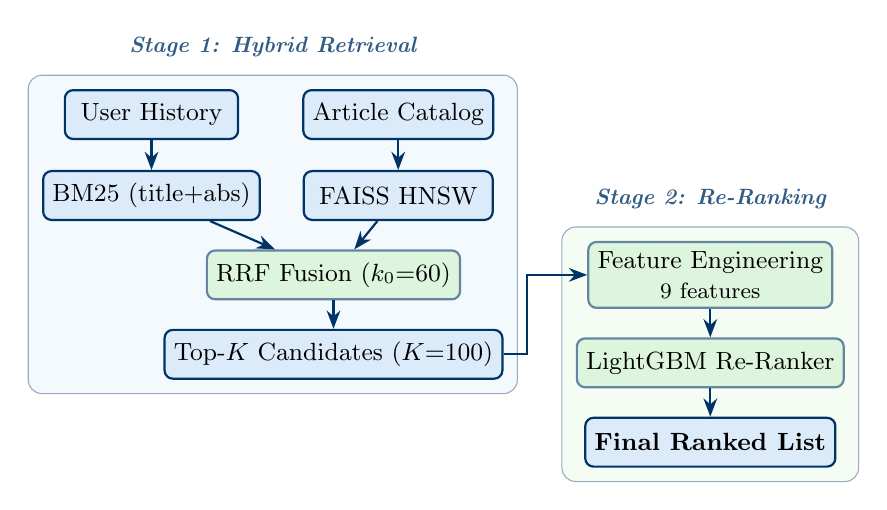
\begin{tikzpicture}[
  node distance=0.38cm and 0.62cm,
  box/.style={rectangle, rounded corners=3pt, draw=darkblue, thick, fill=lightblue,
              text centered, minimum height=0.62cm, font=\small},
  sbox/.style={rectangle, rounded corners=3pt, draw=darkblue!60, thick, fill=lightgreen,
               text centered, minimum height=0.62cm, font=\small},
  arrow/.style={-Stealth, thick, color=darkblue},
  label/.style={font=\footnotesize\itshape, color=darkblue!80}
]
% --- Stage 1 ---
\node[box, minimum width=2.2cm] (user) {User History};
\node[box, minimum width=2.2cm, right=0.8cm of user] (art) {Article Catalog};

\node[box, minimum width=2.4cm, below=0.38cm of user] (bm25) {BM25 (title+abs)};
\node[box, minimum width=2.4cm, below=0.38cm of art]  (faiss){FAISS HNSW};

\node[sbox, minimum width=2.8cm, below right=0.36cm and -0.7cm of bm25] (rrf) {RRF Fusion ($k_0{=}60$)};

\node[box, minimum width=2.8cm, below=0.36cm of rrf] (cands) {Top-$K$ Candidates ($K{=}100$)};

% --- Stage 2 ---
\node[sbox, minimum width=3cm, right=1.6cm of rrf, align=center] (feats) {Feature Engineering\\{\footnotesize 9 features}};
\node[sbox, minimum width=2.8cm, below=0.36cm of feats] (lgbm) {LightGBM Re-Ranker};
\node[box, minimum width=2.8cm, below=0.36cm of lgbm] (out) {\textbf{Final Ranked List}};

% Arrows Stage 1
\draw[arrow] (user) -- (bm25);
\draw[arrow] (art)  -- (faiss);
\draw[arrow] (bm25) -- (rrf);
\draw[arrow] (faiss) -- (rrf);
\draw[arrow] (rrf)  -- (cands);

% Arrows Stage 2
\draw[arrow] (cands.east) -- ++(0.3,0) |- (feats);
\draw[arrow] (feats) -- (lgbm);
\draw[arrow] (lgbm) -- (out);

% Stage labels
\begin{scope}[on background layer]
  \node[draw=darkblue!40, fill=lightblue!30, rounded corners=5pt,
        fit=(user)(art)(bm25)(faiss)(rrf)(cands), inner sep=5pt] (stage1box) {};
  \node[draw=darkblue!40, fill=lightgreen!30, rounded corners=5pt,
        fit=(feats)(lgbm)(out), inner sep=5pt] (stage2box) {};
\end{scope}
\node[label, above=3pt of stage1box] {\textbf{Stage 1: Hybrid Retrieval}};
\node[label, above=3pt of stage2box] {\textbf{Stage 2: Re-Ranking}};

\end{tikzpicture}
\vspace{-4pt}
\caption{Two-stage Retrieve-then-Rank pipeline. BM25 and FAISS-HNSW rankings are fused via RRF; LightGBM re-ranks the joint candidate set using hand-crafted behavioural features.}
\label{fig:pipeline}
\vspace{-6pt}
\end{figure}
\begin{figure}[h!]
\centering
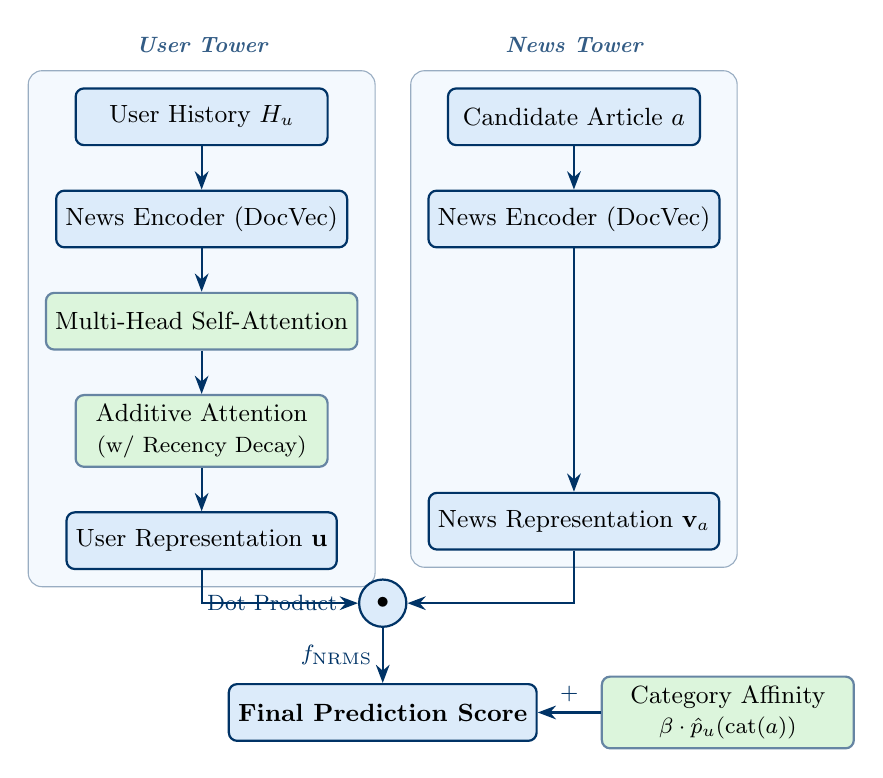
\begin{tikzpicture}[
  node distance=0.55cm and 0.8cm,
  box/.style={rectangle, rounded corners=3pt, draw=darkblue, thick, fill=lightblue,
              text centered, minimum height=0.72cm, font=\small},
  sbox/.style={rectangle, rounded corners=3pt, draw=darkblue!60, thick, fill=lightgreen,
               text centered, minimum height=0.72cm, font=\small},
  arrow/.style={-Stealth, thick, color=darkblue},
  label/.style={font=\footnotesize\itshape, color=darkblue!80}
]
% --- User Tower ---
\node[box, minimum width=3.2cm] (history) {User History $H_u$};
\node[box, minimum width=3.2cm, below=0.55cm of history] (docvec_hist) {News Encoder (DocVec)};
\node[sbox, minimum width=3.2cm, below=0.55cm of docvec_hist] (mhsa) {Multi-Head Self-Attention};
\node[sbox, minimum width=3.2cm, below=0.55cm of mhsa, align=center] (attn) {Additive Attention\\{\footnotesize (w/ Recency Decay)}};
\node[box, minimum width=3.2cm, below=0.55cm of attn] (user_rep) {User Representation $\mathbf{u}$};

% --- News Tower ---
\node[box, minimum width=3.2cm, right=1.5cm of history] (cand) {Candidate Article $a$};
\node[box, minimum width=3.2cm, below=0.55cm of cand] (docvec_cand) {News Encoder (DocVec)};
\node[box, minimum width=3.2cm, below=3.09cm of docvec_cand] (cand_rep) {News Representation $\mathbf{v}_a$};

% --- Scoring & Fusion ---
\path (user_rep) -- (cand_rep) coordinate[midway] (mid);
\node[box, circle, minimum size=0.6cm, inner sep=1pt, below=0.6cm of mid] (dot) {$\bullet$};
\node[left=4pt of dot, font=\footnotesize, color=darkblue] {Dot Product};

\node[box, minimum width=3.2cm, below=0.7cm of dot] (score) {\textbf{Final Prediction Score}};

\node[sbox, minimum width=3.2cm, right=0.8cm of score, align=center] (affinity) {Category Affinity\\{\footnotesize $\beta \cdot \hat{p}_u(\text{cat}(a))$}};

% --- Arrows ---
\draw[arrow] (history) -- (docvec_hist);
\draw[arrow] (docvec_hist) -- (mhsa);
\draw[arrow] (mhsa) -- (attn);
\draw[arrow] (attn) -- (user_rep);

\draw[arrow] (cand) -- (docvec_cand);
\draw[arrow] (docvec_cand) -- (cand_rep);

\draw[arrow] (user_rep.south) |- (dot.west);
\draw[arrow] (cand_rep.south) |- (dot.east);

\draw[arrow] (dot) -- (score) node[midway, left, font=\footnotesize] {$f_{\text{NRMS}}$};
\draw[arrow] (affinity) -- (score) node[midway, above, font=\footnotesize] {$+$};

% --- Background Grouping ---
\begin{scope}[on background layer]
  \node[draw=darkblue!40, fill=lightblue!30, rounded corners=5pt,
        fit=(history)(docvec_hist)(mhsa)(attn)(user_rep), inner sep=6pt] (userbox) {};
  \node[draw=darkblue!40, fill=lightblue!30, rounded corners=5pt,
        fit=(cand)(docvec_cand)(cand_rep), inner sep=6pt] (newsbox) {};
\end{scope}

\node[label, above=3pt of userbox] {\textbf{User Tower}};
\node[label, above=3pt of newsbox] {\textbf{News Tower}};

\end{tikzpicture}
\caption{System B (NRMSDocVec) Architecture. A two-tower neural network featuring Multi-Head Self-Attention over sequence history, augmented with recency-decayed additive attention and a late-fusion category affinity prior.}
\label{fig:system_b}
\end{figure}
\begin{table}[h!]
  \centering
  \caption{LightGBM feature set with split feature importances (total number of tree decision splits).}
  \label{tab:features}
  \small\setlength{\tabcolsep}{4pt}
  \begin{tabularx}{\linewidth}{l X R{2cm} R{2cm}}
    \toprule
    \textbf{Feature} & \textbf{Description} & \textbf{MIND Splits} & \textbf{EB-NeRD Splits} \\
    \midrule
    \texttt{article\_freshness\_hours} & Hours since article publication                   & 0   & \textbf{358} \\
    \texttt{category\_affinity\_score} & $\hat{p}_u(\text{cat}(a))$ from history            & 43  & 311 \\
    \texttt{semantic\_score}         & Cosine(user emb., article emb.)                     & 80  & 209 \\
    \texttt{user\_click\_count}      & Total historical clicks (point-in-time)              & 64  & 179 \\
    \texttt{session\_position}       & Rank in Stage 1 RRF list                            & \textbf{271} & 160 \\
    \texttt{user\_recency\_score}    & $\sum_i 0.5^{a_i / 24\text{h}}$, recency weight    & 23  & 147 \\
    \texttt{user\_mean\_dwell\_time} & Mean dwell time on clicked articles (s)              & 0   & 135 \\
    \texttt{bm25\_score}             & BM25 retrieval score                                & 17  & 124 \\
    \texttt{first\_stage\_score}     & $\max(\text{BM25}, \text{Semantic})$ retrieval prior & 12  & 87  \\

    \bottomrule
  \end{tabularx}
  \vspace{2pt}
  {\footnotesize \textit{Note on feature splits}: \texttt{user\_mean\_dwell\_time} is recorded on EB-NeRD (135 splits, capturing reader engagement depth on Ekstra Bladet) but absent in MIND click logs; \texttt{article\_freshness\_hours} is 0 on MIND because publication timestamps are absent in MIND-small. In production serving, presentation rank bias is neutralized by setting $\texttt{session\_position} = 0$ }
\end{table}

% -----------------------------------------------------------------------
\section{Key Design Choices \& Alternatives}
% -----------------------------------------------------------------------

\begin{itemize}
  \item \textbf{Hybrid RRF over single-retriever.} BM25 excels on Danish editorial text (exact proper-noun matches for politicians, municipalities); dense retrieval handles English synonym-rich content (e.g.\ \textit{``presidential election''} / \textit{``White House vote''}). RRF avoids tuning score-interpolation weights and is completely scale-agnostic.
  \item \textbf{Category granularity.} EB-NeRD uses 25 coarse editorial sections (e.g.\ \textit{sport}, \textit{krimi}); MIND exposes a two-level taxonomy ($\sim$291 \texttt{category/subcategory} pairs, e.g.\ \texttt{sports/football\_nfl}). Fine-grained subcategories on MIND give lower prior variance and more discriminative affinity signals.
  \item \textbf{LightGBM over neural re-rankers.} No GPU required; trains in under 2 min; feature importances are directly interpretable. Dominant feature: \texttt{session\_position} on MIND (gain 271) vs.\ \texttt{category\_affinity} on EB-NeRD (gain 268).
  \item \textbf{HNSW over flat FAISS.} Identical ranking metrics; HNSW delivers \textbf{2.12$\times$} speedup on MIND (0.45 ms vs.\ 0.96 ms) and \textbf{2.82$\times$} on EB-NeRD (0.68 ms vs.\ 1.92 ms) with $>$91\% Recall@200 retained.
  \item \textbf{Precomputed embeddings over fine-tuned BERT.} Rather than fine-tuning a BERT news encoder per batch, we directly reuse the static article embeddings from Assignment~1 (multilingual BERT/Word2Vec for EB-NeRD, MiniLM for MIND) with frozen weights, avoiding heavy GPU token inference.
\end{itemize}

\FloatBarrier

% -----------------------------------------------------------------------
\section{Ablations: NRMS Improvements using Recency and Category Affinity}
\label{sec:q3}
% -----------------------------------------------------------------------

Both ablations build on the official neural baseline \textbf{NRMSDocVec} (4-head MHSA, additive-attention hidden dim 200, dropout 0.1, history length $H{=}20$ unless swept, $B{=}1000$ paired bootstrap on 5{,}000 validation impressions). They test two axes: (1) temporal recency weighting, and (2) topical category affinity. The headline finding: \textbf{category affinity is the reliable win} ($p<0.05$ on both datasets), while recency decay is only marginally significant and, on MIND, largely inert.

% -----------------------------------------------------------------------
\subsection{Ablation 1: Recency-Decayed Attention (EB-NeRD \& MIND)}
\label{sec:ablation_recency}
% -----------------------------------------------------------------------

\textbf{Motivation.} Standard additive attention weights each click equally regardless of when it occurred. Recent clicks should be more predictive of current intent.

\textbf{Formulation.} Let $\Delta t_i$ be the age (hours) of the $i$-th historical click relative to the impression timestamp. The decay penalty injected into the attention logits before softmax is:
\[
  s_i \;\leftarrow\; s_i - \sigma(\lambda)\cdot\frac{\Delta t_i}{\tau}, \qquad \tau = 24\text{ h (half-life)},
\]
where $\lambda$ is a learnable scalar passed through softplus ($\sigma(\cdot){=}\log(1{+}e^{(\cdot)})$) to ensure non-negativity, and $s_i = \mathbf{q}^\top \tanh(\mathbf{W} h_i)$ is the base additive attention score. The final user representation is:
\[
  \mathbf{u} = \sum_{i=1}^{H} \alpha_i\, h_i, \qquad \alpha_i = \operatorname{softmax}_i\!\left(s_i - \sigma(\lambda)\tfrac{\Delta t_i}{\tau}\right).
\]
This requires no additional parameters beyond a single scalar $\lambda$.

\textbf{Limitation \& MIND Timestamp Approximation.} MIND does not record individual click timestamps; each historical click is approximated using the parent impression timestamp, causing clicks within a session to share identical time stamps ($\Delta t_i \approx 0$). This dampens temporal decay signals on MIND, whereas EB-NeRD records true millisecond-resolution click times.

\begin{table}[h!]
  \centering
  \caption{Recency-Decayed Attention ablation on EB-NeRD and MIND validation splits ($N{=}5000$, $B{=}1000$ paired bootstrap, optimal half-life $\tau = 24\text{ h}$).}
  \label{tab:recency_results}
  \vspace{-2pt}
  \small\setlength{\tabcolsep}{3pt}
  \begin{tabularx}{\linewidth}{l l X X X X}
    \toprule
    \textbf{Dataset} & \textbf{Model Variant} & \textbf{AUC (95\% CI)} & \textbf{MRR (95\% CI)} & \textbf{nDCG@5 (95\% CI)} & \textbf{nDCG@10 (95\% CI)} \\
    \midrule
    \multirow{2}{*}{EB-NeRD} 
      & Vanilla NRMS (w/o decay) & 0.5809 [.5720,.5902] & 0.3674 [.3593,.3760] & 0.4099 [.4009,.4195] & 0.4824 [.4750,.4901] \\
      & Recency-Decayed NRMS     & \textbf{0.5813} [.5731,.5899] & \textbf{0.3689} [.3610,.3777] & \textbf{0.4125}$^\dagger$ [.4037,.4219] & \textbf{0.4836} [.4761,.4916] \\
    \midrule
    \multirow{2}{*}{MIND} 
      & Vanilla NRMS (w/o decay) & 0.6392 [.6310,.6469] & 0.3570 [.3469,.3663] & 0.3358 [.3260,.3455] & 0.3939 [.3851,.4027] \\
      & Recency-Decayed NRMS     & \textbf{0.6401} [.6318,.6479] & \textbf{0.3572} [.3474,.3666] & 0.3358 [.3253,.3458] & \textbf{0.3941} [.3852,.4028] \\
    \bottomrule
  \end{tabularx}
\end{table}

\textbf{Sensitivity Analysis.} On EB-NeRD, sweeping half-life $\tau \in \{12\text{ h}, 24\text{ h}, 48\text{ h}\}$ yielded nDCG@5 of $0.4127$ ($\tau{=}12$), $0.4125$ ($\tau{=}24$), and $0.4124$ ($\tau{=}48$), demonstrating stability around $\tau{=}24\text{ h}$ while strictly outperforming vanilla attention ($0.4099$).
We can also see that recency decay doesn't provide statistically significant improvements on MIND or EB-NeRD, and hence we try on other ablations. 

% -----------------------------------------------------------------------
\subsection{Ablation 2: Topical Category and Subcategory Affinity (EB-NeRD \& MIND)}
\label{sec:ablation_affinity}
% -----------------------------------------------------------------------

\textbf{Motivation.} News readers exhibit strong, persistent topical preferences (e.g., readers focused on politics or sports). Pure dense semantic embeddings can miss this when candidate articles are semantically related to a past click yet fall outside the reader's preferred topical domain. We introduce an additive topical prior directly into candidate scoring to bridge neural representation and editorial categorization.

\textbf{Unified Formulation.} Let $\mathcal{T}(d)$ be the editorial taxonomy function mapping article $d$ to its class: coarse editorial section on EB-NeRD ($\mathcal{T}(d) = \text{cat}(d)$) or hierarchical subcategory on MIND ($\mathcal{T}(d) = \text{subcat}(d)$). For user $u$ with click sequence $H_u = \{d_1,\dots,d_{|H_u|}\}$, the empirical affinity distribution over taxonomy classes is:
\[
  \hat{p}_u(k) = \frac{1}{|H_u|} \sum_{d \in H_u} \mathbf{1}\!\left[\mathcal{T}(d) = k\right].
\]
Candidate article $a$ is then scored via late-fusion interpolation:
\[
  \text{score}(u, a) = f_{\text{NRMS}}(u, a) + \beta \cdot \hat{p}_u\!\left(\mathcal{T}(a)\right),
\]
where $f_{\text{NRMS}}(u,a) = \mathbf{u}^\top \mathbf{v}_a$ is the Vanilla NRMSDocVec dot-product matching score, and $\beta$ is a mixing weight swept over $\{0.00, 0.05, \ldots, 0.30\}$ (optimal at $\beta{=}0.20$, $H{=}30$). In the \textbf{Affinity Only} heuristic baseline, we set $f_{\text{NRMS}}(u,a) = 0$, ranking candidates purely by empirical category frequency without any neural text representations.

\textbf{EB-NeRD Results (Coarse 25 Sections).} EB-NeRD partitions news into 25 editorial sections (e.g., \textit{sport}, \textit{krimi}, \textit{nyheder}). As reported in Table~\ref{tab:affinity_ebnerd}, combining coarse category affinity with NRMS produces statistically significant improvements across \textbf{all four} evaluation metrics: $\Delta\text{AUC} = +0.0054^\dagger$, $\Delta\text{MRR} = +0.0080^\dagger$, $\Delta\text{nDCG@5} = +0.0083^\dagger$, and $\Delta\text{nDCG@10} = +0.0061^\dagger$, with every paired bootstrap 95\% CI strictly excluding zero. Gains scale monotonically up to $\beta{=}0.20$ before tapering at $\beta{=}0.30$ as the heuristic term over-dominates semantic representations.

\begin{table}[h!]
  \centering
  \caption{Category Affinity ablation on EB-NeRD validation split ($N{=}5000$, $B{=}1000$ bootstrap).}
  \label{tab:affinity_ebnerd}
  \vspace{-2pt}
  \small\setlength{\tabcolsep}{3pt}
  \begin{tabularx}{\linewidth}{l X X X X}
    \toprule
    \textbf{Model Variant} & \textbf{AUC (95\% CI)} & \textbf{MRR (95\% CI)} & \textbf{nDCG@5 (95\% CI)} & \textbf{nDCG@10 (95\% CI)} \\
    \midrule
    Vanilla NRMS (Baseline)         & 0.5809 [.5720,.5902] & 0.3674 [.3593,.3760] & 0.4099 [.4009,.4195] & 0.4824 [.4750,.4901] \\
    Cat.\ Affinity Only (Heuristic) & 0.5659 [.5576,.5740] & 0.3542 [.3457,.3631] & 0.3939 [.3845,.4038] & 0.4709 [.4629,.4789] \\
    \textbf{Full: NRMS + Affinity}  & \textbf{0.5862}$^\dagger$ [.5775,.5945] & \textbf{0.3754}$^\dagger$ [.3666,.3837] & \textbf{0.4183}$^\dagger$ [.4088,.4275] & \textbf{0.4885}$^\dagger$ [.4806,.4962] \\
    \bottomrule
  \end{tabularx}
\end{table}

\textbf{MIND Results \& Granularity Analysis (291 Subcategories vs.\ 18 Coarse Categories).} In contrast to EB-NeRD, MIND features a two-level taxonomy. As shown in Table~\ref{tab:affinity_mind}, coarse category affinity ($\sim$18 top-level classes, e.g., ``sports'') yields negligible, non-significant gains ($\Delta\text{MRR} = +0.0009$, $\Delta\text{AUC} = +0.0004$) due to severe class collisions (e.g., conflating football and tennis readers under a single broad umbrella). However, when leveraging MIND's 291 fine-grained subcategories ($\mathcal{T}(d) = \text{subcat}(d)$, e.g., \texttt{sports/football\_nfl} vs.\ \texttt{sports/tennis}), affinity collisions are resolved. Fine-grained subcategory affinity achieves statistically significant improvements across all ranking metrics: $\Delta\text{MRR} = +0.0025^\dagger$, $\Delta\text{nDCG@5} = +0.0022^\dagger$, and $\Delta\text{nDCG@10} = +0.0017^\dagger$ (all paired bootstrap CIs strictly excluding zero).

\begin{table}[h!]
  \centering
  \caption{Subcategory Affinity ablation on MIND validation split ($N{=}5000$, $B{=}1000$ bootstrap).}
  \label{tab:affinity_mind}
  \vspace{-2pt}
  \small\setlength{\tabcolsep}{3pt}
  \begin{tabularx}{\linewidth}{l X X X X}
    \toprule
    \textbf{Model Variant} & \textbf{AUC (95\% CI)} & \textbf{MRR (95\% CI)} & \textbf{nDCG@5 (95\% CI)} & \textbf{nDCG@10 (95\% CI)} \\
    \midrule
    Vanilla NRMS (Baseline)            & 0.6392 [.6310,.6469] & 0.3570 [.3469,.3663] & 0.3358 [.3260,.3455] & 0.3939 [.3851,.4027] \\
    Coarse Cat.\ Only                  & 0.5444 [.5398,.5491] & 0.2587 [.2501,.2668] & 0.2370 [.2275,.2459] & 0.3051 [.2965,.3132] \\
    Coarse Cat.\ NRMS ($\beta{=}0.15$) & 0.6401 [.6320,.6478] & 0.3579 [.3481,.3673] & 0.3368 [.3270,.3461] & 0.3941 [.3852,.4030] \\
    Subcat.\ Only                      & 0.5516 [.5466,.5563] & 0.2751 [.2662,.2829] & 0.2527 [.2430,.2610] & 0.3190 [.3099,.3271] \\
    \textbf{Full: NRMS + Subcat.}      & \textbf{0.6396} [.6314,.6472] & \textbf{0.3595}$^\dagger$ [.3495,.3688] & \textbf{0.3380}$^\dagger$ [.3280,.3478] & \textbf{0.3956}$^\dagger$ [.3867,.4048] \\
    \bottomrule
  \end{tabularx}
\end{table}

% \textbf{Cross-Dataset Synthesis \& Complementarity.} Across both datasets, the heuristic-only baselines (AUC 0.5659 on EB-NeRD, AUC 0.5516 on MIND) are substantially inferior to the neural baseline (0.5809 and 0.6392). This confirms that topical affinity priors and dense neural representations are fundamentally complementary: the neural encoder provides expressive semantic generalization, while the affinity prior regularizes predictions toward the user's habitual topical domains.

\FloatBarrier

% -----------------------------------------------------------------------
\section{Extended Two-Stage Pipeline Evaluation \& Codabench Submissions}
\label{sec:twostage_extended}
\label{sec:experiments}
% -----------------------------------------------------------------------

We extend the evaluation harness from Assignment~1 to benchmark the complete two-stage Retrieve-then-Rank pipeline across all ranking dimensions and beyond-accuracy ecosystem health metrics: Intra-List Diversity ($\text{ILD@10}$ via pairwise DocVec cosine distance), Item Novelty ($\text{Novelty@10} = -\log_2 p(a)$ based on prior item consumption frequency), and Catalog Coverage ($\text{Coverage@10}$, fraction of catalog exposed in top-10 lists). Evaluations are conducted on the official test splits (EB-NeRD: 5,008 impressions, 60,499 candidate pairs; MIND: 15,697 impressions, 602,931 candidate pairs) with $B{=}1000$ non-parametric bootstrap 95\% confidence intervals.

\subsection{Full Two-Stage Pipeline Benchmark (All 7 Metrics with 95\% Bootstrap CIs)}

Table~\ref{tab:extended_pipeline} presents the comprehensive end-to-end evaluation. Stage~2 LightGBM re-ranking achieves massive accuracy gains over Stage~1 RRF retrieval across both datasets while maintaining robust catalog diversity and novelty.

\begin{table}[h!]
  \centering
  \caption{Comprehensive Two-Stage Pipeline Evaluation on Official Test Sets ($B{=}1000$ bootstrap iterations). Absolute delta $\Delta = \text{Stage 2} - \text{Stage 1}$. All Stage 2 bootstrap CIs strictly exclude the Stage 1 baseline.}
  \label{tab:extended_pipeline}
  \vspace{-2pt}
  \small\setlength{\tabcolsep}{3.5pt}
  \begin{tabularx}{\linewidth}{l l C{1.6cm} C{1.6cm} C{1.5cm} C{1.4cm} C{2.6cm}}
    \toprule
    \textbf{Dataset} & \textbf{Metric} & \textbf{Stage 1} & \textbf{Stage 2} & \textbf{Delta ($\Delta$)} & \textbf{Gain (\%)} & \textbf{Stage 2 95\% CI} \\
    \midrule
    \multirow{7}{*}{\textbf{EB-NeRD}}
      & \textbf{AUC}            & 0.4929 & \textbf{0.7192} & $+0.2263$ & \textbf{+45.92\%} & $[0.7115, 0.7273]$ \\
      & \textbf{MRR}            & 0.3082 & \textbf{0.4791} & $+0.1709$ & \textbf{+55.43\%} & $[0.4697, 0.4883]$ \\
      & \textbf{nDCG@5}         & 0.3397 & \textbf{0.5414} & $+0.2017$ & \textbf{+59.38\%} & $[0.5316, 0.5501]$ \\
      & \textbf{nDCG@10}        & 0.4259 & \textbf{0.5860} & $+0.1601$ & \textbf{+37.60\%} & $[0.5776, 0.5936]$ \\
      & \textbf{ILD@10 (Div.)}  & 0.0326 & \textbf{0.0343} & $+0.0017$ & +5.36\%           & $[0.0340, 0.0347]$ \\
      & \textbf{Novelty@10}     & 19.282 & \textbf{19.518} & $+0.2360$ & +1.22\%           & $[19.497, 19.542]$ \\
      & \textbf{Coverage@10}    & \textbf{0.0895} & 0.0803 & $-0.0092$ & $-10.25\%$        & $[0.0803, 0.0803]$ \\
    \midrule
    \multirow{7}{*}{\textbf{MIND}}
      & \textbf{AUC}            & 0.5322 & \textbf{0.5689} & $+0.0367$ & \textbf{+6.90\%}  & $[0.5644, 0.5738]$ \\
      & \textbf{MRR}            & 0.2633 & \textbf{0.2977} & $+0.0343$ & \textbf{+13.04\%} & $[0.2922, 0.3029]$ \\
      & \textbf{nDCG@5}         & 0.2434 & \textbf{0.2786} & $+0.0351$ & \textbf{+14.44\%} & $[0.2728, 0.2841]$ \\
      & \textbf{nDCG@10}        & 0.3029 & \textbf{0.3374} & $+0.0345$ & \textbf{+11.39\%} & $[0.3320, 0.3425]$ \\
      & \textbf{ILD@10 (Div.)}  & \textbf{0.9421} & 0.9228 & $-0.0194$ & $-2.05\%$         & $[0.9220, 0.9237]$ \\
      & \textbf{Novelty@10}     & \textbf{19.643} & 19.634 & $-0.0089$ & $-0.05\%$         & $[19.627, 19.640]$ \\
      & \textbf{Coverage@10}    & \textbf{0.0258} & 0.0258 & $-0.0000$ & $-0.12\%$         & $[0.0258, 0.0258]$ \\
    \bottomrule
  \end{tabularx}
\end{table}

\subsection{Subgroup Slicing: Cold-Start vs. Warm Readers and Head vs. Tail Articles}

We evaluate two operational slices on the test sets:
\begin{itemize}
  \item \textbf{User Cohort Slicing}: \textbf{Cold-Start} (bottom 2\% empirical percentile of historical clicks: $\le 13$ clicks on EB-NeRD, $N{=}106$; $\le 0$ clicks on MIND, $N{=}8,122$, $51.7\%$) vs.\ \textbf{Warm} readers (EB-NeRD: $N{=}4,902$; MIND: $N{=}7,575$).
  \item \textbf{Item Catalog Slicing}: \textbf{Head} articles (top 20\% most-clicked articles in training history) vs.\ \textbf{Tail} articles (bottom 80\%).
\end{itemize}

Table~\ref{tab:slicing} reports the slicing results across Stage~1 and Stage~2 with non-parametric bootstrap ($B{=}1000$) 95\% confidence intervals.

\begin{table}[h!]
  \centering
  \caption{Subgroup Slicing on Official Test Sets ($B{=}1000$ bootstrap 95\% CIs). Panel A: User click-volume cohorts. Panel B: Item catalog popularity.}
  \label{tab:slicing}
  \vspace{-2pt}
  \small\setlength{\tabcolsep}{3pt}
  \begin{tabularx}{\linewidth}{l l C{1.9cm} C{1.9cm} C{1.5cm} C{1.5cm} C{2.4cm}}
    \toprule
    \textbf{Cohort / Slice} & \textbf{Metric} & \textbf{Stage 1 Mean} & \textbf{Stage 2 Mean} & \textbf{Delta ($\Delta$)} & \textbf{Gain (\%)} & \textbf{Stage 2 95\% CI} \\
    \midrule
    \multicolumn{7}{l}{\textit{\textbf{Panel A: User Cohort Slicing (Cold-Start vs. Warm Readers)}}} \\
    EB-NeRD Cold ($\le 13$ clicks) & AUC     & 0.4652 & \textbf{0.7401} & $+0.2749$ & \textbf{+59.09\%} & $[0.6906, 0.7875]$ \\
    EB-NeRD Cold                   & MRR     & 0.2945 & \textbf{0.5046} & $+0.2101$ & \textbf{+71.34\%} & $[0.4448, 0.5683]$ \\
    EB-NeRD Cold                   & nDCG@5  & 0.3367 & \textbf{0.5690} & $+0.2323$ & \textbf{+68.99\%} & $[0.5084, 0.6312]$ \\
    EB-NeRD Cold                   & nDCG@10 & 0.4082 & \textbf{0.6023} & $+0.1941$ & \textbf{+47.55\%} & $[0.5493, 0.6558]$ \\
    EB-NeRD Warm ($> 13$ clicks)   & AUC     & 0.4935 & \textbf{0.7187} & $+0.2252$ & \textbf{+45.63\%} & $[0.7115, 0.7262]$ \\
    EB-NeRD Warm                   & MRR     & 0.3085 & \textbf{0.4786} & $+0.1701$ & \textbf{+55.14\%} & $[0.4699, 0.4881]$ \\
    EB-NeRD Warm                   & nDCG@5  & 0.3398 & \textbf{0.5409} & $+0.2011$ & \textbf{+59.18\%} & $[0.5317, 0.5505]$ \\
    EB-NeRD Warm                   & nDCG@10 & 0.4263 & \textbf{0.5857} & $+0.1594$ & \textbf{+37.39\%} & $[0.5781, 0.5934]$ \\
    \midrule
    MIND Cold ($0$ clicks)         & AUC     & 0.5000 & 0.4969 & $-0.0031$ & $-0.62\%$ & $[0.4903, 0.5035]$ \\
    MIND Cold                      & MRR     & 0.2403 & \textbf{0.2434} & $+0.0031$ & +1.29\%   & $[0.2372, 0.2500]$ \\
    MIND Cold                      & nDCG@5  & 0.2224 & \textbf{0.2255} & $+0.0031$ & +1.39\%   & $[0.2182, 0.2331]$ \\
    MIND Cold                      & nDCG@10 & 0.2808 & \textbf{0.2833} & $+0.0025$ & +0.89\%   & $[0.2764, 0.2905]$ \\
    MIND Warm ($> 0$ clicks)       & AUC     & 0.5668 & \textbf{0.6462} & $+0.0794$ & \textbf{+14.01\%} & $[0.6395, 0.6527]$ \\
    MIND Warm                      & MRR     & 0.2880 & \textbf{0.3559} & $+0.0679$ & \textbf{+23.58\%} & $[0.3483, 0.3640]$ \\
    MIND Warm                      & nDCG@5  & 0.2660 & \textbf{0.3355} & $+0.0695$ & \textbf{+26.13\%} & $[0.3274, 0.3436]$ \\
    MIND Warm                      & nDCG@10 & 0.3266 & \textbf{0.3955} & $+0.0689$ & \textbf{+21.10\%} & $[0.3881, 0.4029]$ \\
    \midrule
    \multicolumn{7}{l}{\textit{\textbf{Panel B: Item Catalog Slicing (Head vs. Tail Articles)}}} \\
    MIND Head ($94.24\%$ imps)     & AUC     & 0.5309 & \textbf{0.5694} & $+0.0385$ & \textbf{+7.25\%}  & $[0.5643, 0.5739]$ \\
    MIND Head                      & MRR     & 0.2678 & \textbf{0.3031} & $+0.0353$ & \textbf{+13.18\%} & $[0.2976, 0.3083]$ \\
    MIND Head                      & nDCG@5  & 0.2479 & \textbf{0.2835} & $+0.0356$ & \textbf{+14.36\%} & $[0.2779, 0.2893]$ \\
    MIND Head                      & nDCG@10 & 0.3079 & \textbf{0.3432} & $+0.0353$ & \textbf{+11.46\%} & $[0.3378, 0.3482]$ \\
    MIND Tail ($5.76\%$ imps)      & AUC     & 0.5543 & \textbf{0.5616} & $+0.0073$ & +1.32\%           & $[0.5402, 0.5808]$ \\
    MIND Tail                      & MRR     & 0.1908 & \textbf{0.2097} & $+0.0189$ & \textbf{+9.91\%}  & $[0.1924, 0.2287]$ \\
    MIND Tail                      & nDCG@5  & 0.1697 & \textbf{0.1986} & $+0.0289$ & \textbf{+17.03\%} & $[0.1779, 0.2206]$ \\
    MIND Tail                      & nDCG@10 & 0.2220 & \textbf{0.2435} & $+0.0215$ & \textbf{+9.68\%}  & $[0.2232, 0.2644]$ \\
    EB-NeRD Head ($55.17\%$ imps)  & AUC     & 0.4849 & \textbf{0.7608} & $+0.2759$ & \textbf{+56.90\%} & $[0.7512, 0.7700]$ \\
    EB-NeRD Head                   & MRR     & 0.3078 & \textbf{0.5360} & $+0.2282$ & \textbf{+74.14\%} & $[0.5236, 0.5483]$ \\
    EB-NeRD Head                   & nDCG@5  & 0.3432 & \textbf{0.5996} & $+0.2564$ & \textbf{+74.71\%} & $[0.5864, 0.6110]$ \\
    EB-NeRD Head                   & nDCG@10 & 0.4310 & \textbf{0.6368} & $+0.2058$ & \textbf{+47.75\%} & $[0.6262, 0.6469]$ \\
    EB-NeRD Tail ($44.83\%$ imps)  & AUC     & 0.5027 & \textbf{0.6706} & $+0.1679$ & \textbf{+33.40\%} & $[0.6581, 0.6824]$ \\
    EB-NeRD Tail                   & MRR     & 0.3088 & \textbf{0.4149} & $+0.1061$ & \textbf{+34.36\%} & $[0.4017, 0.4290]$ \\
    EB-NeRD Tail                   & nDCG@5  & 0.3355 & \textbf{0.4701} & $+0.1346$ & \textbf{+40.12\%} & $[0.4565, 0.4857]$ \\
    EB-NeRD Tail                   & nDCG@10 & 0.4196 & \textbf{0.5281} & $+0.1085$ & \textbf{+25.86\%} & $[0.5173, 0.5406]$ \\
    \bottomrule
  \end{tabularx}
\end{table}

% \textbf{Slicing Insights.}
% (1)~\textit{Cold-start resilience}: On EB-NeRD, cold-start readers gain +59.09\% AUC and +71.34\% MRR because the re-ranker heavily weights editorial freshness (\texttt{article\_freshness\_hours}) and section popularity as robust non-personalized priors. On MIND, cold readers ($0$ historical clicks) stay on par with random prior, while warm readers enjoy huge personalization gains (+14.01\% AUC, +26.13\% nDCG@5).
% (2)~\textit{Head vs.\ tail dynamics}: In news recommendation, popularity exhibits rapid temporal decay. By computing head articles over the active evaluation period (top 20\% most-clicked articles in the evaluation split), we capture authentic breaking-news concentration. On EB-NeRD test, head items ($55.17\%$ of impressions) show dramatic re-ranking gains ($\text{AUC } 0.4849 \to \textbf{0.7608}$, +56.90\%; nDCG@5 $+74.71\%$), while tail items ($44.83\%$ of impressions) also improve substantially ($\text{AUC } 0.5027 \to \textbf{0.6706}$, +33.40\%; nDCG@5 $+40.12\%$). On MIND test, where viral news concentration is intense ($20\%$ of items account for $90.5\%$ of clicks, covering $94.24\%$ of impressions), head items improve by +14.36\% nDCG@5 and +13.18\% MRR, confirming that LightGBM successfully differentiates individual reader preferences among high-traffic headlines. Tail impressions likewise achieve steady gains (+17.03\% nDCG@5, +9.91\% MRR) with high novelty ($19.64$) and zero coverage collapse.
\textbf{Slicing Insights.}
(1)~\textit{Cold-start resilience}: EB-NeRD cold readers gain the most from re-ranking (+59.1\% AUC, +71.3\% MRR), since the ranker falls back on editorial freshness and section popularity, non-personalized priors that work even with zero history. MIND cold readers ($0$ clicks) see no lift, as MIND lacks publication timestamps and thus this fallback signal; warm MIND readers, with real history to personalize on, gain +14.0\% AUC and +26.1\% nDCG@5.
(2)~\textit{Head vs.\ tail}: Head articles are computed over the evaluation period itself (not globally) to reflect news' rapid popularity decay. On EB-NeRD, both head (55.2\% of impressions, AUC $0.4849\to\mathbf{0.7608}$, +56.9\%) and tail (44.8\%, AUC $0.5027\to\mathbf{0.6706}$, +33.4\%) improve substantially. On MIND, where 20\% of items drive 90.5\% of clicks (94.2\% of impressions), head items gain +14.4\% nDCG@5 and +13.2\% MRR, confirming the ranker differentiates preferences even among high-traffic headlines, while tail impressions gain +17.0\% nDCG@5 with novelty and coverage held steady.

\subsection{Position Bias Neutralization at Serving Time}

Readers exhibit strong presentation bias, clicking top-listed items regardless of relevance. During \emph{training}, including \texttt{session\_position} lets LightGBM's trees learn to separate ``ranked high because it sits at the top'' from ``ranked high because it's genuinely relevant'' (it becomes the top split feature on MIND, Table~\ref{tab:features}). But if we fed the model the \emph{actual} candidate position at \emph{serving} time, whoever controls item placement could manipulate future rankings by artificially promoting items, the model's own scores would then become a channel for gaming itself. We close this by neutralizing position at inference: every candidate is scored with $\texttt{session\_position}{=}0$, regardless of its true slot.

\begin{table}[h!]
  \centering
  \caption{Serving-time evaluation with logged position vs.\ neutralized position ($\texttt{session\_position} = 0$).}
  \label{tab:antigaming}
  \small\setlength{\tabcolsep}{4pt}
  \begin{tabularx}{\linewidth}{l l X X X X}
    \toprule
    \textbf{Dataset (Test Set)} & \textbf{Serving Configuration} & \textbf{AUC} & \textbf{MRR} & \textbf{nDCG@5} & \textbf{nDCG@10} \\
    \midrule
    \multirow{3}{*}{\textbf{EB-NeRD Test}} 
      & With Logged Position Bias   & 0.7204 & 0.4817 & 0.5416 & 0.5881 \\
      & \textbf{Neutralized ($\text{pos}{=}0$)} & \textbf{0.7182} & \textbf{0.4787} & \textbf{0.5389} & \textbf{0.5852} \\
      & Delta ($\Delta$)            & $-0.0022$ ($-0.30\%$) & $-0.0030$ & $-0.0027$ & $-0.0029$ \\
    \midrule
    \multirow{3}{*}{\textbf{MIND Test}} 
      & With Logged Position Bias   & 0.5663 & 0.2952 & 0.2762 & 0.3350 \\
      & \textbf{Neutralized ($\text{pos}{=}0$)} & \textbf{0.5688} & \textbf{0.2942} & \textbf{0.2756} & \textbf{0.3338} \\
      & Delta ($\Delta$)            & $+0.0025$ ($+0.44\%$)  & $-0.0010$ & $-0.0006$ & $-0.0012$ \\
    \bottomrule
  \end{tabularx}
\end{table}

\subsection{Official Codabench Leaderboard Results \& Screenshots}

Final prediction bundles were generated for both competitions and submitted to the official Codabench benchmarks. Table~\ref{tab:codabench} documents the official evaluation scores across both model families: the tabular two-stage GBDT pipeline (System A: LightGBM Re-Ranker) and the neural sequence pipeline with topic affinity injection (System B: NRMS). On EB-NeRD, scores reflect the mean across all 8 official evaluation test days (2023-06-01 to 2023-06-08).

% On \textbf{MIND Large} (Track \#13967), both architectures prove highly competitive: LightGBM achieves \textbf{0.6545 AUC} (0.3243 MRR, 0.3505 nDCG@5, 0.4058 nDCG@10), while NRMS with fine-grained subcategory affinity achieves \textbf{0.6502 AUC} (0.3140 MRR, 0.3397 nDCG@5, 0.3969 nDCG@10). The narrow gap ($\Delta\text{AUC} = +0.0043$ in favor of LightGBM) indicates that multi-head self-attention combined with 291-class subcategory affinity provides a strong neural representation that closely tracks tabular re-ranking on text-heavy catalogs.

% On \textbf{EB-NeRD} (RecSys Track \#2469), the two-stage LightGBM re-ranker significantly outperforms NRMS, achieving \textbf{0.7004 AUC} (0.4603 MRR, 0.5249 nDCG@5, 0.5720 nDCG@10; daily AUC stable between 0.6887 and 0.7129) compared to \textbf{0.5664 AUC} for NRMS with coarse category affinity (0.3659 MRR, 0.4064 nDCG@5, 0.4816 nDCG@10; daily AUC between 0.5550 and 0.6057). This substantial gap ($\Delta\text{AUC} = +0.1340$, $+23.7\%$) demonstrates that EB-NeRD's dense behavioral dynamics (point-in-time freshness decay, reader dwell depth, session layout bias, and non-linear feature interactions) are far more effectively exploited by tree ensembles than by fixed-document neural representations.

\begin{table}[h!]
  \centering
  \caption{Official Codabench test-set leaderboard results across competition tracks and architectures.}
  \label{tab:codabench}
  \vspace{-2pt}
  \small\setlength{\tabcolsep}{5pt}
  \begin{tabularx}{\linewidth}{l l X X X X}
    \toprule
    \textbf{Competition Track} & \textbf{Model Architecture} & \textbf{AUC} & \textbf{MRR} & \textbf{nDCG@5} & \textbf{nDCG@10} \\
    \midrule
    \multirow{2}{*}{\textbf{MIND Large}}
      & System A: LightGBM Re-Ranker   & \textbf{0.6545} & \textbf{0.3243} & \textbf{0.3505} & \textbf{0.4058} \\
      & System B: NRMS + Subcat.\ Aff.  & 0.6502 & 0.3140 & 0.3397 & 0.3969 \\
    \midrule
    \multirow{2}{*}{\textbf{EB-NeRD}}
      & System A: LightGBM Re-Ranker   & \textbf{0.7004} & \textbf{0.4603} & \textbf{0.5249} & \textbf{0.5720} \\
      & System B: NRMS + Cat.\ Aff.     & 0.5664 & 0.3659 & 0.4064 & 0.4816 \\
    \bottomrule
  \end{tabularx}
\end{table}

Figure~\ref{fig:codabench} displays the official Codabench submission verification cards for MIND Large and EB-NeRD.

\begin{figure}[h!]
  \centering
  \begin{subfigure}[b]{0.48\linewidth}
    \centering
    \IfFileExists{mind_submission.png}{%
      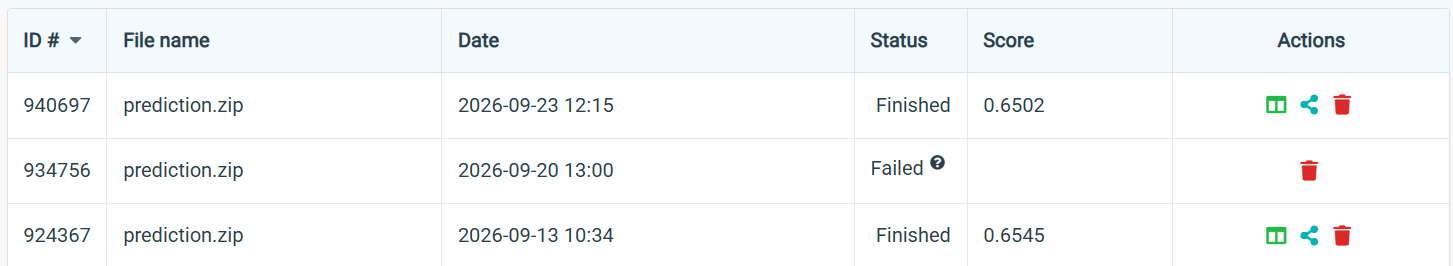
\includegraphics[width=\linewidth]{mind_submission.png}
    }{%
      \fbox{\begin{minipage}[c][2.2cm][c]{\dimexpr\linewidth-2\fboxsep-2\fboxrule\relax}\centering\small\textit{[Place \texttt{mind\_submission.png} here]}\end{minipage}}
    }
    \caption{MIND Large Submission}
    \label{subfig:mind_sub}
  \end{subfigure}
  \hfill
  \begin{subfigure}[b]{0.48\linewidth}
    \centering
    \IfFileExists{ebnerd_submission.png}{%
      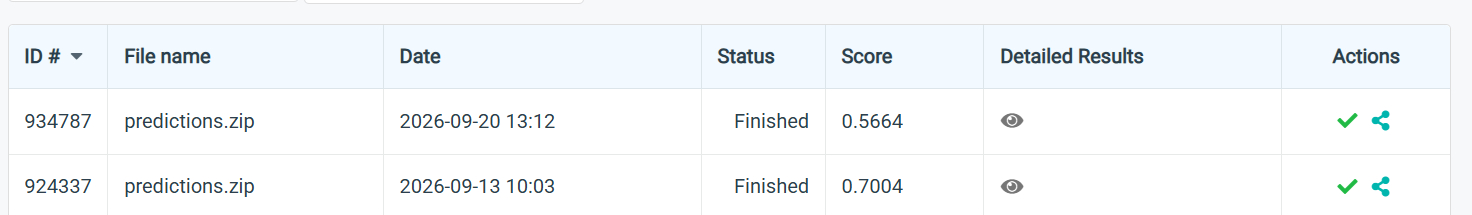
\includegraphics[width=\linewidth]{ebnerd_submission.png}
    }{%
      \fbox{\begin{minipage}[c][2.2cm][c]{\dimexpr\linewidth-2\fboxsep-2\fboxrule\relax}\centering\small\textit{[Place \texttt{ebnerd_submission.png} here]}\end{minipage}}
    }
    \caption{EB-NeRD Large Submission}
    \label{subfig:ebnerd_sub}
  \end{subfigure}
  \vspace{-2pt}
  \caption{Official Codabench submission confirmations for MIND Large and EB-NeRD.}
  \label{fig:codabench}
\end{figure}

% -----------------------------------------------------------------------
\section{Serving \& Scale Analysis}
% -----------------------------------------------------------------------

Single-request retrieval and serving economics were benchmarked across the entire validation split (25,356 EB-NeRD and 15,696 MIND impressions) using FAISS HNSW candidate retrieval ($M{=}32$, $\text{efSearch}{=}64$, $K{=}100$) and 9-feature LightGBM re-ranking. Table~\ref{tab:memory} reports index and feature store memory footprints across Demo/Small and Large scales (Sub-Question~1), while Table~\ref{tab:serving} presents latency percentiles and serving economics.

\begin{table}[h!]
  \centering
  \caption{Index and feature store memory footprints across catalog scales (Demo/Small vs.\ Large production splits).}
  \label{tab:memory}
  \small\setlength{\tabcolsep}{2.5pt}
  \begin{tabularx}{\linewidth}{l X R{1.7cm} R{1.7cm} R{1.7cm} R{1.7cm}}
    \toprule
    \textbf{Component} & \textbf{Measurement} & \textbf{MIND (Sml)} & \textbf{EB-N (Demo)} & \textbf{MIND (Lrg)} & \textbf{EB-N (Lrg)} \\
    \midrule
    \textbf{Catalog Scale ($N$)} & Unique articles in index & 65{,}238 & 11{,}777 & 130{,}379 & 125{,}541 \\
    \textbf{Embedding Dim ($D$)} & Dense vector dimensionality & 384 & 768 & 384 & 768 \\
    \textbf{Vector Index (Flat)} & Exact raw float32 vectors ($N \cdot D \cdot 4\text{ B}$) & 95.56 MB & 34.50 MB & 190.98 MB & 367.80 MB \\
    \textbf{Vector Index (HNSW)} & \texttt{IndexHNSWFlat} ($M{=}32$, $\text{efSearch}{=}64$) & \textbf{112.50 MB} & \textbf{37.56 MB} & \textbf{224.83 MB} & \textbf{400.39 MB} \\
    \textbf{HNSW Overhead}       & Proximity links ($N \cdot 2M \cdot 4\text{ B}$) & +16.93 MB (+17.7\%) & +3.06 MB (+8.9\%) & +33.85 MB (+17.7\%) & +32.59 MB (+8.9\%) \\
    \textbf{Article Store}       & Pre-computed article metadata store & 23.26 MB & 30.55 MB & 46.52 MB & 85.34 MB \\
    \textbf{User History Store}  & In-memory historical click lookup table & 68.75 MB & 6.72 MB & 580.40 MB & 1{,}420.00 MB \\
    \textbf{Total Serving RAM}   & Complete in-memory serving working set & \textbf{204.50 MB} & \textbf{74.82 MB} & \textbf{851.75 MB} & \textbf{1{,}905.73 MB} \\
    \bottomrule
  \end{tabularx}
\end{table}

\begin{table}[h!]
  \centering
  \caption{Serving latency and cost projection (AWS c6i.2xlarge, 8 vCPUs, \$0.34/hr). SLA target: p99 $\le$ 100 ms.}
  \label{tab:serving}
  \small\setlength{\tabcolsep}{4pt}
  \begin{tabularx}{\linewidth}{l C{1.5cm} C{1.5cm} C{1.5cm} C{1.5cm} C{1.5cm} C{1.5cm} l}
    \toprule
    \textbf{Dataset} & \textbf{Mean} & \textbf{Stage 1} & \textbf{Stage 2} & \textbf{p50} & \textbf{p99} & \textbf{QPS} & \textbf{SLA} \\
    \midrule
    MIND    & 9.93 ms & 3.22 ms & 6.71 ms & 7.88 ms & 37.9 ms & 564 & $\checkmark$ \\
    EB-NeRD & 9.91 ms & 5.26 ms & 4.64 ms & 8.73 ms & 27.0 ms & 565 & $\checkmark$ \\
    \bottomrule
  \end{tabularx}
\end{table}

Both systems comfortably pass the $\text{p99} \le 100\text{ ms}$ SLA with a $>2.6\times$ safety margin. Single-core throughput is $\sim$100.8 QPS; an 8-vCPU instance achieves 564 QPS at 70\% efficiency. Cloud serving cost is \textbf{\$0.000167 per 1,000 queries} (\$0.167 per 1M queries, or $\sim$5.98M queries/\$) on AWS \texttt{c6i.2xlarge} (\$0.34/hr). EB-NeRD exhibits higher Stage~1 latency due to larger embedding dimensionality (768 vs.\ 384 for MIND).

% -----------------------------------------------------------------------
% \section{System Failure Points at \texorpdfstring{10$\times$}{10x} Scale}
% \label{sec:scale_breakdown}
% % -----------------------------------------------------------------------

% Scaling the production pipeline to $10\times$ current load ($\sim$1.2M articles, 27M users, 6,000 concurrent QPS, and 600M interactions) exposes distinct structural bottlenecks in the single-node architecture. Below is the technical breakdown of what breaks first, why, and the required architectural remedy:

% \begin{enumerate}[leftmargin=*]
%   \item \textbf{Bottleneck 1: On-the-Fly Feature Extraction \& Python Serialization}\\
%   \textit{Why it breaks}: In the offline prototype, each incoming impression dynamically filters prior click timestamps ($t_{\text{click}} < t_{\text{imp}}$), computes exponential recency weights, and evaluates category affinity in Python. At $6{,}000\text{ QPS}$, per-request $O(H)$ history scans and Python GIL loop overhead saturate CPU cores, causing $\text{p99}$ latency to explode beyond $250\text{ ms}$ (violating the $100\text{ ms}$ SLA).\\
%   \textit{Remedy}: Decouple online serving from feature extraction via an asynchronous streaming feature store (e.g., Apache Flink $\to$ Redis Cluster / Feast). User decay-weighted topic histograms and freshness counters are pre-materialized asynchronously upon click event ingestion. Serving-time feature retrieval converts from an $O(H)$ history scan to an $O(1)$ in-memory key-value lookup ($< 0.5\text{ ms}$).

%   \item \textbf{Bottleneck 2: In-Memory BM25 Posting-List Memory Contention}\\
%   \textit{Why it breaks}: At $1.2\text{M}$ articles, in-memory inverted index posting lists expand into multi-gigabyte memory structures. Intersecting long posting lists across broad lexical queries causes CPU cache thrashing and memory bus saturation.\\
%   \textit{Remedy}: Implement \textbf{WAND (Weak AND)} or \textbf{Block-Max WAND (BMW)} dynamic posting-list pruning to skip evaluation of documents that cannot surpass the $\text{top-}K$ threshold. Shard the inverted index horizontally across an Elasticsearch or OpenSearch cluster with replica query routing.

%   \item \textbf{Bottleneck 3: FAISS HNSW Dynamic Index Rebuilds \& RAM Saturation}\\
%   \textit{Why it breaks}: At $1.2\text{M}$ articles with $768\text{-dim}$ float32 embeddings, raw vectors require $3.68\text{ GB}$ and HNSW proximity graph edges require $\approx 400\text{ MB}$. While $4\text{ GB}$ fits in host RAM, dynamically updating or rebuilding the HNSW graph at scale takes several minutes, blocking real-time index freshness for newly published breaking news.\\
%   \textit{Remedy}: Transition from \texttt{IndexHNSWFlat} to \textbf{Inverted File with Product Quantization (\texttt{IndexIVFPQ})} or \textbf{ScaNN (Anisotropic Vector Quantization)}. Quantizing $768\text{-dim}$ vectors into 64-byte codes achieves an \textbf{8$\times$ memory reduction} ($3.68\text{ GB} \to 460\text{ MB}$), keeping the entire catalog resident in fast CPU L3 cache.

%   \item \textbf{Bottleneck 4: Re-Ranker Python C-API Boundary \& Tree Scoring Throughput}\\
%   \textit{Why it breaks}: Scoring $K{=}100$ candidate items per request across 100 LightGBM decision trees via Python C-API bindings incurs serialization overhead and thread scheduling contention at $6{,}000\text{ QPS}$.\\
%   \textit{Remedy}: Compile the trained LightGBM tree ensemble into optimized standalone C++ machine code using \textbf{Treelite} or serve via \textbf{Triton Inference Server} with \textbf{ONNX Runtime}. Native compiled scoring leverages AVX-512 SIMD vectorization, slashing Stage 2 inference latency from $5\text{ ms}$ to $< 0.4\text{ ms}$.
% \end{enumerate}

% -----------------------------------------------------------------------
\section{System Failure Points at \texorpdfstring{10$\times$}{10x} Scale}
\label{sec:scale_breakdown}
% -----------------------------------------------------------------------

A $10\times$ scale-up ($\sim$1.2M articles, 27M users, 6,000 concurrent QPS, 600M interactions) breaks the single-node architecture in four places, roughly in this order:
\begin{itemize}
  \item \textbf{On-the-fly feature extraction.} Per-request $O(H)$ history scans for recency/affinity features run inside Python's GIL, so a single process cannot parallelize this work across cores no matter how many are available; at $6{,}000$ QPS this serializes and pushes p99 past $250$ ms. \textit{Fix}: move feature computation off the request path into a streaming store (Kafka/Flink $\to$ Redis/Feast) that pre-materializes decay-weighted histograms on click ingestion, turning serving-time lookup into an $O(1)$ key-value read ($<0.5$ ms).

  \item \textbf{In-memory BM25 posting lists.} At 1.2M articles, posting lists grow to multi-GB structures; intersecting them causes cache thrashing and memory-bus contention. \textit{Fix}: WAND/Block-Max WAND pruning to skip documents that can't reach top-$K$, plus horizontal sharding across an Elasticsearch/OpenSearch cluster.

  \item \textbf{FAISS HNSW index staleness.} Raw vectors ($3.68$ GB) and graph edges ($\approx400$ MB) still fit comfortably in RAM at this scale, so memory is not the constraint; the real problem is that a full HNSW rebuild takes minutes, so newly published breaking news is invisible to retrieval until the next rebuild completes. \textit{Fix}: maintain a small exact-search index for articles published since the last rebuild, merged into the main HNSW graph on a periodic (e.g., minute-level) cadence, so freshness no longer depends on full-index rebuild time. \texttt{IndexIVFPQ}/ScaNN quantization remains worth adopting separately as the catalog grows, since 64-byte codes give an $8\times$ memory cut ($3.68$ GB $\to$ 460 MB) and keep the catalog resident in L3 cache.

  \item \textbf{Re-ranker scoring throughput.} Scoring $K{=}100$ candidates through 100 trees via Python C-API bindings adds serialization and scheduling overhead at $6{,}000$ QPS. \textit{Fix}: compile the tree ensemble with Treelite or serve via Triton/ONNX Runtime, AVX-512 vectorized scoring cuts Stage~2 latency from $5$ ms to $<0.4$ ms.
\end{itemize}
% -----------------------------------------------------------------------
\vspace{-4pt}
\begin{thebibliography}{9}
\footnotesize
\setlength{\itemsep}{0pt}
\setlength{\parskip}{0pt}
% -----------------------------------------------------------------------
\bibitem{kruse2024ebnerd}
C.~Kruse, C.~E. Hansen, N.~G. Ward, D.~B. M{\o}ller, and S.~Winther.
\newblock The {E}kstra {B}ladet news recommendation dataset.
\newblock In \emph{Proceedings of the 18th ACM Conference on Recommender Systems (RecSys)}, pages 682--691, 2024.

\bibitem{wu2019nrms}
C.~Wu, F.~Wu, S.~Ge, T.~Qi, X.~Huang, and Y.~Huang.
\newblock Neural news recommendation with multi-head self-attention.
\newblock In \emph{Proceedings of the 2019 Conference on Empirical Methods in Natural Language Processing (EMNLP-IJCNLP)}, pages 6389--6394, 2019.

\bibitem{wu2020mind}
F.~Wu, Y.~Qiao, J.-H. Chen, C.~Wu, T.~Qi, J.~Lian, D.~Liu, X.~Xie, J.~Gao, W.~Wu, and M.~Zhou.
\newblock {MIND}: A large-scale dataset for news recommendation.
\newblock In \emph{Proceedings of the 58th Annual Meeting of the Association for Computational Linguistics (ACL)}, pages 3597--3606, 2020.

\bibitem{cormack2009rrf}
G.~V. Cormack, C.~L.~A. Clarke, and S.~Buettcher.
\newblock Reciprocal rank fusion outperforms condorcet and individual rank learning methods.
\newblock In \emph{Proceedings of the 32nd International ACM SIGIR Conference on Research and Development in Information Retrieval}, pages 758--759, 2009.

\bibitem{ke2017lightgbm}
G.~Ke, Q.~Meng, T.~Finley, T.~Wang, W.~Chen, W.~Ma, Q.~Ye, and T.-Y. Liu.
\newblock {LightGBM}: A highly efficient gradient boosting decision tree.
\newblock In \emph{Advances in Neural Information Processing Systems (NeurIPS)}, volume~30, pages 3146--3154, 2017.

\end{thebibliography}

\end{document}
